\documentclass[book]{jlreq}

\usepackage{graphicx}
\usepackage{amsmath,amssymb,amsthm}
\usepackage{mathtools}
%%\usepackage{siunitx}
\usepackage{physics}
\usepackage{bm}

\renewcommand{\today}{\the\year/\the\month/\the\day}
\renewcommand{\contentsname}{Contents}
\renewcommand{\refname}{References}
%%\renewcommand{\figurename}{Fig.~}
\renewcommand{\tablename}{Table~}

\begin{document}
\title{Low-Level Radio Frequency Systems}
\author{Shin-ichi YOSHIMOTO}
\maketitle
\tableofcontents
%%\clearpage

%%\part{数学的準備}
\chapter{Introduction}

\chapter{RF Control Strategy}
\chapter{RF System Models}

LLRFシステムの設計と解析には、RFシステムの(数学的)モデルが不可欠である。ここでいうモデルとは、RFシステムの出力と入力の間の(動的な)関係を伝達関数の形で記述したものです。伝達関数は、RF システムの動作と制限に関する洞察を与えます。例えば、RF ドライブ、ビーム負荷、および外部擾乱(電磁ノイズ、熱ドリフト、機械振動など)がある場合の RF システムの出力を、伝達関数を使用して予測することができます。また、モデルから得られる有用な情報として、ループ位相、ループゲイン、ループ遅延の安定限界値があり、これはRFコントローラのこれらの動作パラメータを決定するのに役立ちます。このように、RFシステムモデルは物理的な原理によって導き出されるため、動作パラメータの最適化やRFシステムの特性の特定にも利用することができます。

\section{一般的な前提条件}

本章で説明するモデルは、RF システムの構成要素の入出力関係(図\ref{Fig3.1}参照)に焦点を当て,それによって RF システムの制御と運用のための設計を可能にするものです。RF 空胴はモデル化される主要なコンポーネントとなります。空洞の入出力は、RF 駆動電力とビームに印加される RF 電界の包絡線によって表現される。空胴における高周波磁場の詳細な空間分布は、入出力関係に関係しないため、議論しない。本章では、RF 系は線形系としてモデル化し、非線形効果については7章で取り上げる。制御系の解析・設計では線形モデルの方が単純である。実際には、加速器の RF 系には非線形成分(RF アンプやクライストロンなど)が存在する。しかし、RFシステムの動作点付近の小さな範囲を考えるならば、線形モデルが良い近似となる。さらに、空洞の駆動項であるRF駆動電力やビームローディングは、モデル化においてノイズレスとして扱われる。Chap.6では、ノイズの多いRF駆動パワーとビームローディングが空洞フィールドに与える影響について議論する予定である。
%
\begin{figure}[hbt]
    \begin{center}
      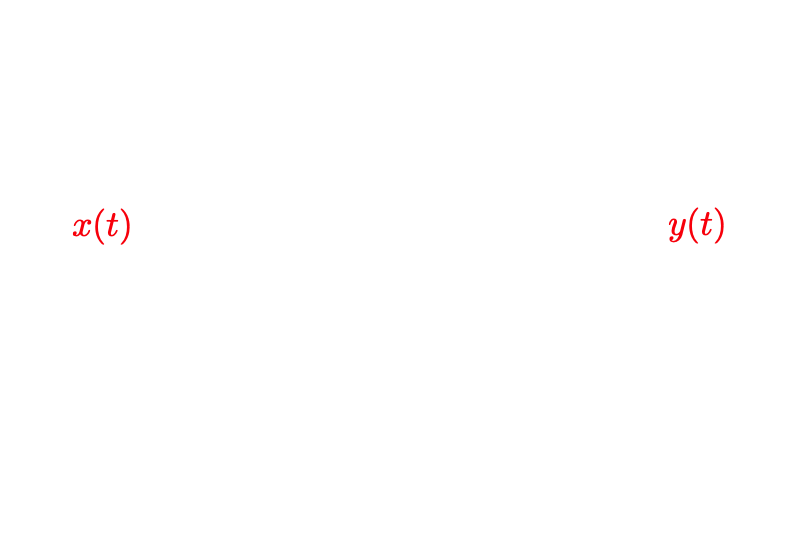
\includegraphics[width=12cm,clip]{figs/Fig3.1.png}
      \caption{入出力関係に注目したRFシステムモデル}
     \label{Fig3.1}
    \end{center}
\end{figure}

加速器 RF システムは、一般的に固定周波数またはゆっくりと時間的に変化する周波数で動作する狭帯域のものである。同期システムから提供されるRF基準信号は、ローカルオシレータ(LO)、クロック、RF動作周波数など、RFステーション内の様々な周波数のソースとして使用される。ここでは、RF基準信号の周波数をRF基準周波数と定義し、それを表すのに$\omega_{ref}$を使用する。デフォルトでは、RF局の実際の動作周波数であるRF動作周波数$\omega_{RF}$は、$\omega_{ref}$に等しいと仮定します。もう 1 つの概念は、キャリア周波数 $\omega_{c}$で、これは柔軟に選択され、多くの場合 $\omega_c = \omega_{RF}$ を選択します。異なるRF信号の場合、$\omega_c$はそれらの共通項を表し、RF成分の入出力関係を記述する際には省略される。$\omega_c = \omega_{RF}$ とすると、RFシステムのモデルをその入出力の包絡線から求めることができる。

$\omega_{RF}$ が定数の場合、$\omega_c$ は$\omega_{RF}$と同じように定義するのが便利ですが、時間的に変化する$\omega_{RF}$ の場合、$\omega_c$ を2通りの方法で扱うことができます。

\begin{enumerate}
    \item $\omega_c$ を変化させて $\omega_{RF}$ に追従させることができます。この方法は、RFシステムモデルにとって$\omega_{RF}$の変化を透過的にし、したがって、RF信号のエンベロープ(すなわちベースバンド信号)のみを扱うことになります。
    \item 固定の $\omega_c$ を選択してもよい。これにより、RFシステムモデルが扱う信号には、時変位相 $\phi (t) = [\omega_{RF} (t)\omega_{c}]t + \phi_{0i}$ ($\varphi_{0i}$ は各信号の定数)が発生する。この方法を用いる場合、RF成分の正しい入出力関係を得るためには、すべてのRF信号の位相の時間変化項 $[\omega_{RF}(t) - \omega_{c}]t$を省略する必要がある。
\end{enumerate}

上記の最初のケースは、RF信号のスペクトルを直接DC付近にシフトさせ、2番目のケースは中間周波数(IF)付近にシフトさせるものです。本書では、RFシステムのモデリングとコントローラ設計を簡単にするために、常に $\omega_c = \omega_{RF}$ を仮定します。

もうひとつの仮定は、加速器の RF システムの帯域幅が RF 動作周波数よりもはるかに小さいという事実から来ている($\omega_{1/2} \ll \omega_{RF}$ 、ここで $\omega_{1/2}$ は全帯域幅の半分)。これは、RF 信号のエンベロープが RF 周波数よりはるかに遅く変化することを意味する。したがって、RF信号の包絡線は、RF周波数の数周期内でほぼ一定として扱うことができる。

\section{RF モデリング方法}

図\ref{Fig3.1}のRFコンポーネントの入出力関係は、時間領域の関数 $g(t) : x(t) \rightarrow y(t)$ として記述することができる。ここで $g$ は静的システムではスカラー($x$ または $y$ がベクトルの場合は行列)、動的システムでは微分方程式(またはその群)である。
ラプラス変換を用いると$g(t)$は$Y(s) = G(s)X(s)$を満たす伝達関数$G(s)$として記述することができ、ここで$X(s)$と$Y(s)$は時間領域の入力と出力信号のラプラス変換である:$X(s) = \mathcal{L}\{x(t)\},\; Y(s) = \mathcal{L}\{y(t)\}$。
演算子$\mathcal{L}\{\cdot\}$ はラプラス変換を表す。ここで、$t<0$のとき$x(t) = 0$、$y(t) = 0$ と仮定した。変数$s$は$s \coloneqq \sigma + j\omega$ として定義される複素周波数である。ここでは、信号のラプラス変換と伝達関数の集まりを周波数領域($s$領域)という言葉で表すことにする。$s$の複素平面を$s$平面と呼ぶ。ラプラス変換は線形システムをモデル化する強力なツールであり、古典的な制御理論の基礎を形成している(Dorf and Bishop 2010)。システムの入力と出力が実数値を持つ時間領域のスカラーである実信号の場合、システムの伝達関数は実数値の係数を持ち、その周波数特性は正と負の周波数に対して対称である。

これまで述べてきたように、RFコンポーネントの入出力信号には同じ搬送波周波数項が含まれており、入出力関係には有用な情報が得られない。そこで、入力信号と出力信号の包絡線から得られる伝達関数のみを考慮することにします。そのために、搬送波周波数項を取り除き、RF信号を位相(複素信号)として記述する。位相とRF信号の変換は、LLRFシステムにおけるRF信号の検出・作動処理とよく一致する。入出力の位相子にラプラス変換を適用すると、複素数値の係数を持ち、非対称な周波数応答を持つ伝達関数が得られる(Novotny and Wouterse 1976\cite{Novotny}; Martin 2004; Harnefors 2007; Brandt 2007; Troeng 2019)。位相から派生したこのような伝達関数には、RFシステムモデルの次数を2から1に減らすことができるという第一の利点があります。後に、LLRFシステムの解析と設計を大幅に簡略化できることがわかります。

\subsection{RF信号の説明}

搬送波の周波数$\omega_c$、時間的に変化する振幅$x_0(t)$と位相$\varphi(t)$を持つRF信号は、時間領域で次のように記述することができる。
%
\begin{equation}
    x(t) = x_0(t) \cdot \cos(\omega_c t + \varphi (t))
    \label{eq:3.1}
\end{equation}
%
ここで、振幅と位相は、RFシステムの動的挙動のモデリングに関連するすべての情報を含んでいる。オイラーの式$e^{j\theta} = \cos\theta + j \sin\theta$から、複素時間領域信号は、上記の信号を虚部としてのサイン項$j x_0(t) \sin (\omega_c t + \varphi (t))$で展開することにより定義され、次のようになる。
%
\begin{equation}
    \tilde{\vb{x}}(t) \coloneqq x_0(t) e^{j(\omega_c t+\varphi(t))}
    \label{eq:3.2}
\end{equation}
%
搬送波周波数項 $e^{j\omega_c t}$は、すべてのRF信号で同じである。$\omega_c = \omega_{RF}$ と $\omega_{RF}$ は定数であるか、RF システムの時定数に比べればゆっくり変化するので、定数として扱うことができる。$e^{j\omega_c t}$を捨てることで、振幅と位相の情報をすべて保持したRF信号の複素包絡線を得ることができる。
%
\begin{equation}
    \vb{x(t)} \coloneqq x_0(t) e^{j\varphi t} = I(t) + j Q(t)
    \label{eq:3.3} 
\end{equation}
%
複素エンベロープ(\ref{eq:3.3})は、「位相ベクトル」の略でフェーザ表示と呼ばれます。その大きさと位相は、それぞれ信号(\ref{eq:3.1})の振幅と位相に対応します。本書では、RF信号をフェーザで表現することにします。

なお,フェーザ表示は特定の$\omega_c$に対して定義されています。異なるキャリア周波数$\omega_c^{\prime}$を使用する場合、(\ref{eq:3.1}) を $x(t) = x_0(t)\cdot \cos(\omega_c^{\prime} t + (\omega_c - \omega_c^{\prime}) t + \varphi (t))$と書き直すことができ、フェーザ表示は$\bm{x(t)}^{\prime} = x_0(t) e^{j (\omega_c - \omega_c^{\prime}) + j \varphi (t)}$となります、
キャリア周波数が$\omega_{RF}$と異なる場合、位相$\varphi^{\prime} (t) = (\omega_c - \omega_c^{\prime}) + \varphi (t)$の振動項が残っていることがわかります。つまり、RF 信号をベースバンドに変換する代わりに、中間周波数$\omega_{IF} = \omega_c - \omega_c^{\prime}$に変換しています。

\subsection{Principle of RF Signal Detection}

LLRFシステムでは、RFディテクタがRF信号を位相に変換し、RFアクチュエータが位相をRF信号に変換します。RFコントローラでは、RFディテクタで測定されたRFフィールドのフェーザーを処理し、RFアクチュエータへの駆動フェーザーを生成します。位相の物理的な意味を理解するために、RF検出器と作動のプロセスを見てみましょう。RFアクチュエーションは、RF検出器の逆プロセスであるため、図\ref{Fig3.2}のI/Q復調器を用いたRF検出の原理のみを分析する。

\begin{figure}[hbt]
    \begin{center}
      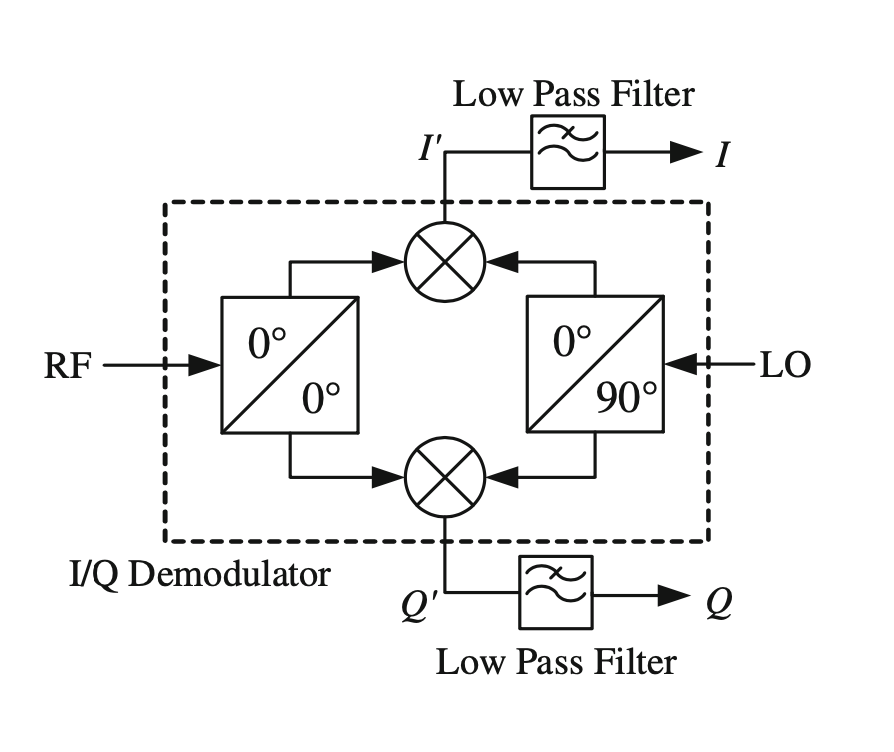
\includegraphics[width=12cm,clip]{figs/Fig3.2.png}
      \caption{A typical RF detector using an I/Q demodulator}
     \label{Fig3.2}
    \end{center}
\end{figure}

空洞からピックアップしたRF信号のフェーザーを検出するために、リファレンスとして局部発振器(LO)を導入する。RF信号とLO信号は次のように表される。
%
\begin{equation}
    x_{RF}(t) = x_{RF0}\cos(\omega_{RF} t+\varphi), \quad  x_{LO}(t) = x_{LO0}\cos(\omega_{LO} t)\notag
\end{equation}
%
ここで、LO位相は0に正規化され、LO周波数$\omega_{LO} < \omega_{RF}$とする。I/Q復調器は、実信号と複素信号の乗算器として動作します。RF信号は同相分配器で分割され、実信号$x'_{RF} = x_{RF}/\sqrt{2}$と等価となります。一方、LO信号は直交スプリッタで分割され、等価な複素信号
%
\begin{equation}
    \tilde{\vb{x}}^{\prime}_{LO} = \frac{x_{LO0}}{\sqrt{2}}[\cos(\omega_{LO} t) -j\sin(\omega_{LO} t)] 
    = \frac{x_{LO0}}{\sqrt{2}} e^{-j\omega_{LO} t}\notag
\end{equation}
%
を形成する。ここで、$0^{\circ}$と$90^{\circ}$の枝はそれぞれ実部と虚部である。$x_{RF}'$のスペクトルは正負の周波数に対して対称であるのに対し、$\tilde{\vb{x}}^{\prime}_{LO}$のスペクトルは負の周波数にのみ現れることに注意してください(図\ref{Fig3.3}参照)。I/Q復調器出力は$x_{RF}'$と$\tilde{\vb{x}}^{\prime}_{LO}$の積であり、次式で与えられます。
%
\begin{equation}
    I^{\prime}(t) + j Q^{\prime}(t) = \frac{x_{RF}x_{LO0}}{4}\left ( e^{-j[(\omega_{RF}+\omega_{LO})t+\varphi]}\right )
    + \left ( e^{j[(\omega_{RF}-\omega_{LO})t+\varphi]}\right )
    \label{eq:3.4}
\end{equation}
%
これらは、それぞれ、$-(\omega_{RF} + \omega_{LO})$と$(\omega_{RF} - \omega_{LO})$の2つの周波数成分を含んでいます。実際には、ローパスフィルタで$-(\omega_{RF} + \omega_{LO})$の周波数成分をフィルタリングし、結果、時間的に変化するフェーザー
%
\begin{equation}
    \vb{x}_{RF}(t) = I(t) + j Q(t) = \frac{x_{RF}x_{LO0}}{4}e^{j[(\omega_{RF}-\omega_{LO})t+\varphi]}
    \label{eq:3.5}
\end{equation}
%
を生成する。図\ref{Fig3.3}の周波数関係から、RF信号のスペクトルから次のようにしてフェーザースペクトルを導出することができます。まず、周波数の原点をLO周波数にシフトし、次に$-(\omega_{RF} + \omega_{LO})$の周波数成分をフィルタリングで除去します。
%
\begin{figure}[hbt]
    \begin{center}
      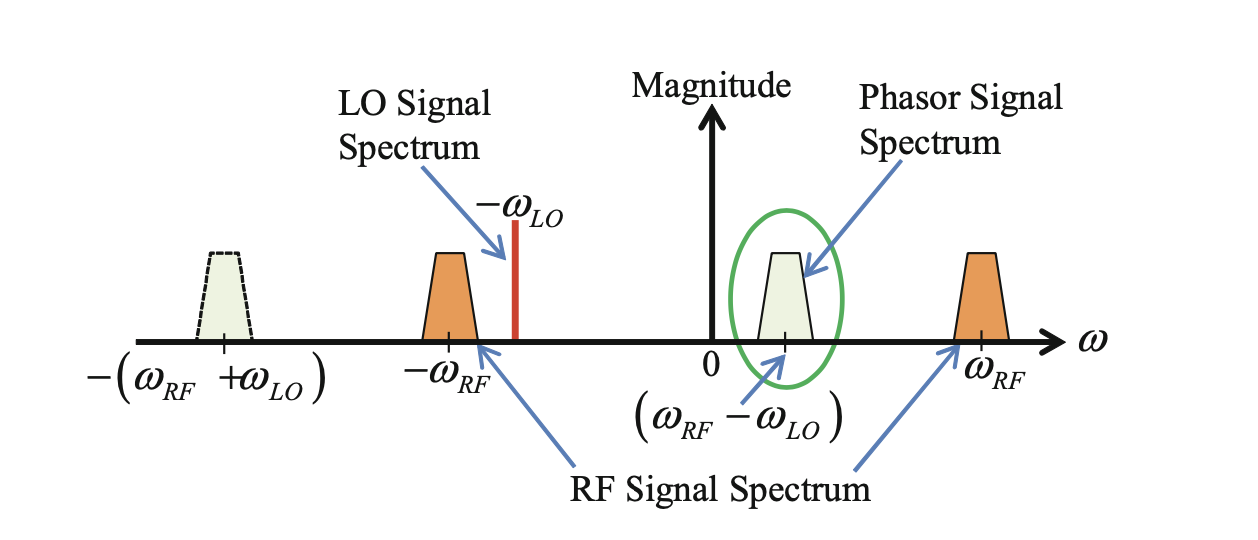
\includegraphics[width=12cm,clip]{figs/Fig3.3.png}
      \caption{RF検波の周波数領域変換。RF検出器の出力は、非対称なスペクトルを持つRF信号の時間変化するフェイザーである。プロットでは、正の周波数で丸で囲んだ部分のみを含むフェーザル・スペクトルになる}
     \label{Fig3.3}
    \end{center}
\end{figure}
%
\begin{figure}[hbt]
    \begin{center}
      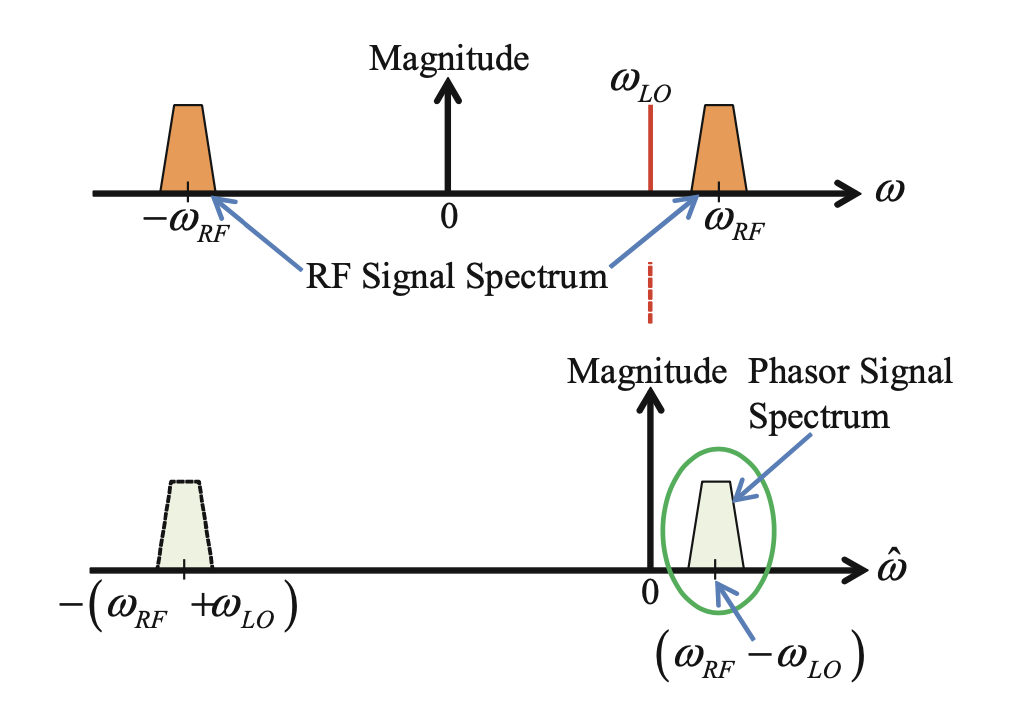
\includegraphics[width=12cm,clip]{figs/Fig3.4.png}
      \caption{Derive the phasor spectrum from the RF signal spectrum}
     \label{Fig3.4}
    \end{center}
\end{figure}
%
図\ref{Fig3.4}を参照してください。これは、新しい周波数$\hat{\omega}=\omega - \omega_{LO}$を定義し、RF信号のゆっくりと変化する包絡線(つまり、新しい周波数領域における低周波成分)だけを維持することに相当する。入力RF信号のスペクトルのサイドバンドの1つをフィルタリングすると、その大きさの半分を失うことになることに注意してください。これは、正弦信号のフーリエ変換と逆フーリエ変換で説明できる。振幅$A$、周波数$\omega_{RF}$の正弦信号のスペクトルは、$\omega_{RF}$に2つの成分を含んでいます。この2つのスペクトル線は、同じ大きさ$A/2$(フーリエ変換の定義によっては係数$2\pi$)で互いに共役です(ただし、この係数は逆変換するときに補正されます)。逆フーリエ変換により、この2本のスペクトル線を使って元のサイン信号を復元することができます。しかし、片方のスペクトル線を捨てて逆フーリエ変換を行うと、再構成される信号の振幅は元の信号の半分にしかなりません。このことから、高周波成分を除去した場合の信号レベルを維持するためには、位相スペクトルの大きさを2倍にする必要がある。

また、周波数シフトは、RF信号のラプラス変換に適用して、対応するフェーザのラプラス変換を得ることができる。RFシステムコンポーネントの伝達関数も、シフトされた周波数に対応して調整されることになる。

\subsection{フェーザ表示のラプラス変換}

粒子加速器のRFシステムの入出力はRF信号である。図\ref{Fig3.1}のモデルでも搬送波の項があるが、、フェーザ表示(包絡線)による入出力関係の方がより興味深い。
フェーザ表示(\ref{eq:3.3})のラプラス変換を導くために、(\refeq{eq:3.2})をラプラス変換すると、次のようになる。
%
\begin{equation}
    \tilde{\vb{X}}(s) = \mathcal{L}\{\tilde{\vb{x}}(t)\} = X(s)\left( 1+j e^{-s\pi / (2\omega_c)}\right)
    \label{eq:3.6}
\end{equation}
%
ただし、$X(s)$は(\ref{eq:3.1})のRF信号$x(t)$をラプラス変換したものである。ここでは、RF信号の1周期内の振幅と位相の変動が無視できる場合、$x(t-\pi/(2\omega_c)) \approx x_0(t)\sin(\omega_c t + \varphi(t))$という近似式を用いている。RFコンポーネントの入出力信号を(\ref{eq:3.2})のような複素時間領域信号で表すと、そのラプラス変換も$\tilde{\vb{Y}}(s) = G(s)\tilde{\vb{X}}(s)$を満足します。ただし、$G(s)$はRFコンポーネントの伝達関数。 図 3.4 によれば、元の RF 信号のスペクトルから、周波数の原点を$\omega_c$ずらし、高い周波数成分を除去することで、フェーザのスペクトルを導出することができます。同様に、$s$平面の周波数軸を$\omega_c$だけずらすと、フェーザラプラス変換という新しい形のラプラス変換が得られます。そして、RFコンポーネントの入力と出力をフェーザラプラス変換の形で記述し、RFコンポーネントを単一入力単一出力(SISO)位相伝達関数としてモデル化することができる。フェーザラプラス変換は新しい複素周波数$\hat{s}\coloneqq\sigma+j\hat{\omega}$ を定義し、$\hat{\omega}\coloneqq\omega-\omega_c$ は RF 信号包絡線の周波数であるシフトした周波数である。$\hat{s}=s-j\omega_c$という関係があります。ここでは、信号の位相伝達関数と位相ラプラス変換の集まりをオフセット周波数領域 ($\hat{s}$領域) という用語で表現する。$\hat{s}$の複素平面を$\hat{s}$平面と呼ぶことにする。

複素包絡線(\ref{eq:3.3})と複素RF信号(\ref{eq:3.2})の関係は、$\vb{x}(t) e^{j\omega_c t} = \tilde{\vb{x}}(t)$と書くことができる。両辺をラプラス変換すると$\vb{X}(s-j\omega_c) = \tilde{\vb{X}}(s)$が得られる、ただし、$\vb{X}(s) = \mathcal{L}\{\vb{x}(t)\}$。独立変数$s$の代わりに$s=\hat{s} + j\omega_c$を使うと、次のようになる。
%
\begin{equation}
    \vb{X}(\hat{s})=\tilde{\vb{X}}(\hat{s}+j\omega_c)=X(\hat{s}+j\omega_c)\left (1+j e^{-(\hat{s}+j\omega_c)\pi/(2\omega_c)} \right )
    \label{eq:3.7}
\end{equation}
%
ただし、指数項は$e^{-\hat{s}\pi/(2\omega_c)}e^{-j\pi/2}$と書くことができる。RF信号の包絡線の搬送波周波数に対する低周波の変化、つまり$ |\hat{s}| \ll \omega_c$だけを考えると$e^{-\hat{s}\pi/(2\omega_c)}\approx 1$ となり、(\ref{eq:3.7})のRF信号のフェーザ・ラプラス変換は次のように簡略化されます。
%
\begin{equation}
    \vb{X}(\hat{s}) \approx 2 X(s)\mid_{s=\hat{s}+j\omega_c}, \quad |\hat{s}| \ll \omega_c
    \label{eq:3.8}
\end{equation}
%
この係数2は、周波数をずらして高い周波数成分を捨てた後の、大きさの半分の損失を補うもので、図 3.3 および 3.4 の議論と一致する。$\vb{Y}(s) = G(s)\vb{X}(s)$ の関係を$\hat{s}$領域に変換すると、$\tilde{\vb{Y}}(\hat{s}+j\omega_c) = G(\hat{s}+j\omega_c)\tilde{\vb{X}}(\hat{s}+j\omega_c)$、さらに (3.7) により$\vb{Y}(\hat{s}) = G(\hat{s}+j\omega_c)\vb{X}(\hat{S})$ が得られます。したがって、フェーザ伝達関数は次のように定義できます。
%
\begin{equation}
    \vb{G}(\hat{s}) \coloneqq G(\hat{s}+j\omega_c) = G(s)\mid_{s=\hat{s}+j\omega_c}, \quad \quad |\hat{s}| \ll \omega_c
    \label{eq:3.9}
\end{equation}
%
したがって、入力と出力のRF信号のフェーザラプラス変換の関係は、次式で与えられる。
%
\begin{eqnarray}
    \vb{Y}(\hat{s}) = \vb{G}(\hat{s}) \vb{X}(\hat{s})
    \label{eq:3.10}
\end{eqnarray}
%
$\vb{G}(\hat{s})$は通常$|\hat{s}|\ll \omega_c$の仮定で適用される。つまり、$\vb{G}(\hat{s})$の低周波 ($\hat{s}$領域)のダイナミクスのほうに興味があり、高周波のモードは無視されていることに注意する。式(\ref{eq:3.8}, \ref{eq:3.9}, \ref{eq:3.10})は,フェイザーラプラス変換に基づく RFシステムのモデリング手法の基礎となるものである。この方法では、RF信号の包絡線をフェーザラプラス変換で記述し、フェーザ伝達関数を用いてRFシステムの挙動をモデル化する。図\ref{Fig3.5}に示すように、$s$平面の実軸を$j\omega_c$に移動させれば$\hat{s}$平面を得ることができる。このような処理を行うと、システムの力学的な性質が変化する。たとえば、$s$面上に2つの共役極$p_1$と$p_2$がある場合、つまり$s$領域に2次系があるとします。これを$\hat{s}$平面に変換すると、2つの極$\hat{p}_1$と$\hat{p}_2$は実軸に対して対称でなくなり、2つの異なる力学モードが生じます。極$\hat{p}_1$は入出力エンベロープの振る舞いを表す低い周波数$(\omega - \omega_c)$であり、$\hat{p}_2$は高い周波数$(\omega + \omega_c)$である。我々は高速時変項には興味がなく、包絡線にのみ興味があるので、位相伝達関数では$\hat{p}_2$ を捨てることにする。これは、$s$領域の2次伝達関数を1次のフェーザ伝達関数で置き換えることができることを意味している。

\begin{figure}[hbt]
    \begin{center}
      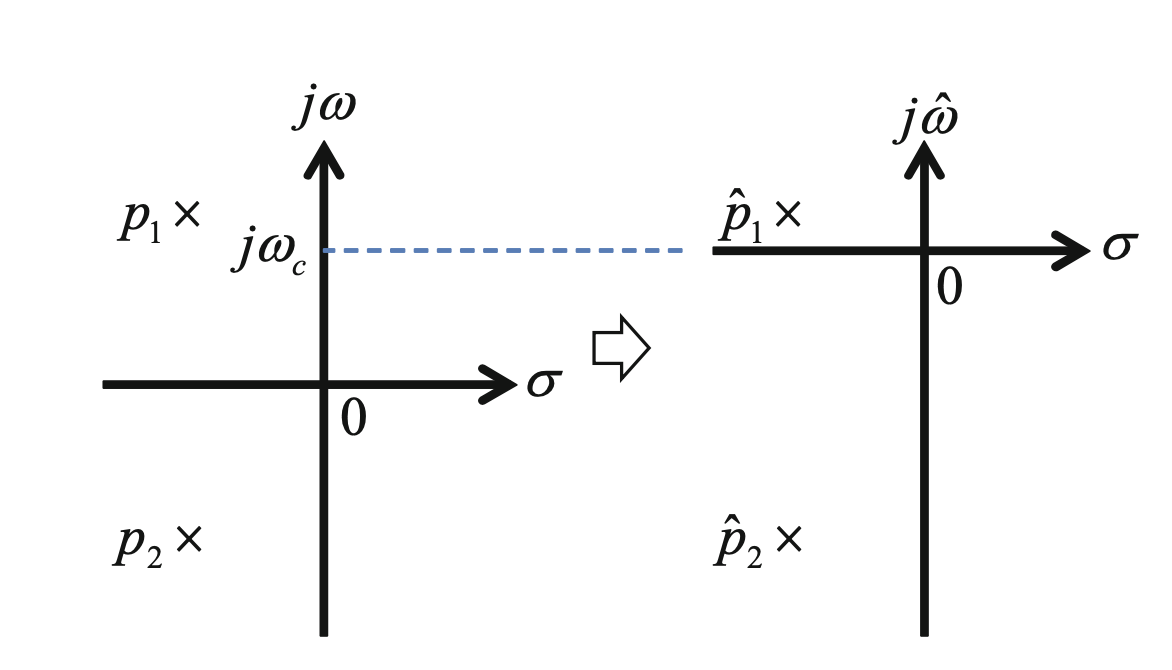
\includegraphics[width=12cm,clip]{figs/Fig3.5.png}
      \caption{Transfer from $s$ plane to $\hat{s}$ plane}
     \label{Fig3.5}
    \end{center}
\end{figure}

RFシステムまたはRF信号のいずれかが搬送波周波数と比較して狭帯域である場合、以下の手順でRFシステムをモデル化することができます。
%
\begin{enumerate}
    \item RFシステムの微分方程式から伝達関数を導出し、$s$を$\hat{s}+j\omega_c$に置き換えて、フェーザ伝達関数を求めます。システムの帯域幅よりはるかに高い周波数での位相伝達関数のダイナミクスは無視する必要があります。
    \item 入力RF信号のラプラス変換を導出し、$s$を$\hat{s}+j\omega_c$に置き換えて2倍し、フェーザラプラス変換を得る。システム帯域幅よりはるかに高い周波数でのRF信号のフェーザラプラス変換の周波数成分は、無視する必要があります。
    \item (\ref{eq:3.10})を用いて、出力RF信号のフェーザラプラス変換を計算する。逆ラプラス変換により、時間領域での出力位相が構築できます。
\end{enumerate}
%
フェイザー伝達関数$\vb{G}(\hat{s})$は複素数の係数を含むことがあり、Matlabのような既存のソフトウェアツールではうまくサポートされないことがあることに注意してください。しかし、実部と虚部を分離することで、2\times2の多入力多出力(MIMO)システムに簡単に変換することができ、ソフトウェアツールにうまく適合させることができます。この場合、入力信号と出力信号はともにフェーザーの実部と虚部を表すI/Qベクトルとして記述する必要があります。システム伝達関数の以下の形式は(\ref{eq:3.10})と等価である。
%
\begin{equation}
    \begin{bmatrix}
        Y_I(\hat{s})\\
        Y_Q(\hat{s})
    \end{bmatrix}
    =
    \begin{bmatrix}
        G_{11}(\hat{s}) & G_{12}(\hat{s}) \\
        G_{21}(\hat(s)) & G_{22}(\hat{s})
    \end{bmatrix}
    \begin{bmatrix}
        X_I(\hat{s}) \\
        X_Q(\hat{s})
    \end{bmatrix}
    \label{eq:3.11}
\end{equation}
%
ここで$G_{11}, G_{12}, G_{21}, G_{22}$は実数係数のみを含み、$\vb{Y}(\hat{s}) = Y_I(\hat{s}) + j Y_Q(\hat{s}), \; \vb{X}(\hat{s}) = X_I(\hat{s}) + j X_Q(\hat{s})$である。MIMO 形式は数値シミュレーションに適している。一方、(\ref{eq:3.10})はRFシステムの動作や特性を解析的に研究するのに有効です。表現を簡単にするため、意味が明確な場合は式中の独立変数$s, \hat{s}, t$を省略する。

\section{Single-Cell Cavity Model}

単セル定在波キャビティは、ストレージリングに広く使用されている。このセクションでは、シングルセルキャビティの電気的、機械的特性の両方をモデル化する。RF駆動電力、ビーム負荷、外乱の存在下での空洞の挙動を研究する。シングルセル空洞のモデルは、マルチセルキャビティの解析のための基礎にもなります。マルチセルキャビティは複数の通過帯域モードを持ち、各モードはシングルセルキャビティと同様の伝達関数で記述することができる。マルチセルキャビティについては、次節で説明する。

\subsection{Parallel RLC Circuit Model}


\begin{thebibliography}{9}
    \bibitem{Novotny}
    Novotny DW, Wouterse JH (1976) Induction machine transfer function and dynamic response by means of complex time variables. IEEE Trans Power App Syst 95(4):1325–1335. https://doi.org/10.1109/T-PAS.1976.32227
    \bibitem{llrf}
    S. Simrock, Z. Geng, Low-Level Radio Frequency Systems, Springer (2022)
    \bibitem{Schilcher}
    T. Schilcher Vector sum control of pulsed accelerating fields in Lorentz force detuned superconducting cavities (1998).
    \bibitem{Wilson}
    P. B. Wilson, High energy electron linacs; application to storage ring RF systems and linear colliders (1987)
\end{thebibliography}
%
%
\end{document}